\documentclass[proof]{beamer}
\usetheme{default}

\usecolortheme{rose}
\usepackage[english]{babel}
\usepackage[utf8]{inputenc}
%\usepackage[latin1]{inputenc}
 \usepackage{amssymb}
 \usepackage{latexsym}
 \usepackage{amsmath}
 \usepackage{amssymb}
 \usepackage{tikz}
 \usepackage{tikz-cd}
\usepackage{array}
\usepackage{rotating}
\usepackage{forest}
\usepackage{color}
\usepackage[all,cmtip]{xy}

\usepackage{pgfplots}
\usepackage{array}
    \newcolumntype{C}{>{\centering\arraybackslash}c}


\definecolor{qbblue}{RGB}{43,126,128}
\definecolor{qborange}{RGB}{242,151,36}
\definecolor{qblight}{RGB}{210,210,210}
\definecolor{qbdark}{RGB}{180,180,180}
\definecolor{qbred}{RGB}{184,13,72}

\setbeamercolor{title}{fg=black}
\setbeamercolor{section in toc}{fg=black}
\setbeamercolor{block title}{bg=qblight,fg=black}
\setbeamercolor{frametitle}{bg=qblight,fg=black}
\setbeamercolor{section in head/foot}{bg=black}
\setbeamertemplate{itemize item}{\color{qbdark}$\blacktriangleright$}
\setbeamertemplate{itemize subitem}{\color{qbdark}$\blacktriangleright$}
%\setbeamercolor*{palette tertiary}{bg=black}
\setbeamercolor{local structure}{fg=black}

\usepackage[style=verbose,backend=biber]{biblatex}
\addbibresource{biblio.bib}

\renewcommand{\_}{\rule{.6em}{.5pt}\hspace{0.023cm}}

\newcommand{\bloc}[2]{\begin{block}{#1}\setlength\abovedisplayskip{0pt}#2\end{block}}

\setbeamertemplate{navigation symbols}{} 
\addtobeamertemplate{footline}{\hfill{\tiny \insertframenumber}\hspace{2em} \vspace{1em}}

\newcommand{\red}[1]{\textcolor{qbred}{#1}}
\newcommand{\blue}[1]{\textcolor{qbblue}{#1}}
\newcommand{\orange}[1]{\textcolor{qborange}{#1}}

\newcommand{\D}{\mathbb{D}}

%\newcommand{\trunc}[1]{|| #1 ||}

\AtBeginSection[]
{
 \begin{frame}<beamer>
 \frametitle{Outline}
 \tableofcontents[currentsection]
 \end{frame}
}

\begin{document}


%\abovedisplayskip=0.0cm
%\abovedisplayshortskip=-0.3cm
%\belowdisplayskip=0.6cm


\title{\red{Differential Geometry in Synthetic Algebraic Geometry}}
\author{Hugo Moeneclaey\\
j.w.w Felix Cherubini, Matthias Hutzler and David Wärn}
\date{\blue{HoTT-UF 2024}\\
Leuven}



\frame{\titlepage}




\frame{\frametitle{Overview}

\bloc{Goal}{
Import \red{differential geometry} tools to \red{synthetic algebraic geometry}.
}

\bloc{Draft}{
\url{https://felix-cherubini.de/diffgeo.pdf}
}

\pause

\bloc{Today}{
Focus on \red{smoothness} for affine schemes.

Give examples of \red{synthetic proofs}.
}

\pause

\begin{center}
\begin{tabular}{ccc}
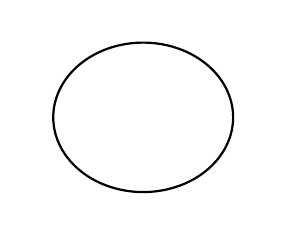
\begin{tikzpicture}[scale=0.4]
  \begin{axis}[
  	axis line style={draw=none},
	tick style={draw=none}, 
	xticklabel=\empty, 
	yticklabel=\empty,
  	restrict y to domain = 0:360,
    	restrict x to domain = 0:360]
\addplot[domain=0:360,data cs=polar, samples=300, line width=2pt] 
(x,{0.4/(sqrt(0.4-0.3*cos(x)*cos(x)))});
  \end{axis}
\end{tikzpicture}
& 
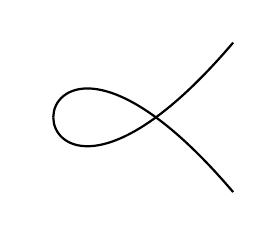
\begin{tikzpicture}[scale=0.4]
  \begin{axis}[
  	axis line style={draw=none},
	tick style={draw=none}, 
	xticklabel=\empty, 
	yticklabel=\empty,
  	restrict y to domain = -1:1,
    	restrict x to domain = -1:1,]
    \addplot [domain = -1:1, samples = 300, line width=2pt]
      {sqrt(x^2*(x+1))};
    \addplot [domain = -1:1, samples = 300, line width=2pt]
      {-sqrt(x^2*(x+1))}; 
  \end{axis}
\end{tikzpicture} 
&
\begin{tikzpicture}[scale=0.4]
  \begin{axis}[
  	axis line style={draw=none},
	tick style={draw=none}, 
	xticklabel=\empty, 
	yticklabel=\empty,
  	restrict y to domain = -1:1,
    	restrict x to domain = -1:1]
    \addplot [domain = -1:1, samples = 300, line width=2pt]
      ({x^2},{x^3});
  \end{axis}
\end{tikzpicture}\\
\blue{Smooth} & \blue{Not smooth} & \blue{Not smooth}
\end{tabular}
\end{center}

}


 \begin{frame}<beamer>
 \frametitle{Outline}
 \tableofcontents
 \end{frame}



\section{Synthetic algebraic geometry}

\frame{\frametitle{What is synthetic algebraic geometry?}

It consists of HoTT plus 3 axioms:

\pause

\bloc{Axiom 1}{
There is a \red{local ring $R$}.
}

\pause

$R$ is a set.

}

\frame{\frametitle{Affine schemes}

For $A$ a finitely presented algebra, we define:
\[Spec(A) = Hom_{Alg}(A,R)\]

\pause

\bloc{Example}{
If:
\[A = R[X]/P\]
then:
\[Spec(A) = \{x:R\ |\ P(x) = 0\}\]
}

\pause

%\bloc{Definition}{
%An affine scheme is a type of the form $Spec(A)$ for some f.p.\ algebra $A$.
%}

\bloc{Definition}{
A type $X$ is an \red{affine scheme} if there is an f.p.\ algebra $A$ such that:
\vspace{-0.1cm}
\[X=Spec(A)\]
}

}

\frame{

\bloc{Axiom 2: \red{Duality}}{
For any f.p.\ algebra $A$ the map:

\[A \to R^{Spec(A)}\]
is an equivalence.
}

\pause

Then:
\begin{itemize}
\item $Spec : \{f.p.\ algebras\} \simeq \{Affine\ schemes\}$
\pause
\item All maps between affine schemes are polynomials.
\end{itemize}

}

\frame{

\bloc{Axiom 3: \red{Zariski local choice}}{
Affine schemes enjoys a weakening of the axiom of choice.
}

}

%\frame{\frametitle{Intuitions behind the axioms}

%\bloc{Idea (conjecture)}{
%Justify these axioms by interpreting HoTT into the higher topos of higher Zariski sheaves.
%}

%$R$ being local has nothing to do with the base ring, it comes from the Zariski topology.

%}

\section{Smoothness for arbitrary types}

\frame{\frametitle{Closed propositions}

\bloc{Definition}{
A proposition $P$ is \red{closed} if there exist $r_1,\hdots,r_n:R$ such that:
\vspace{0.32cm}
\[P \leftrightarrow (r_1=0\land\hdots\land r_n=0)\]
}

\pause

%\bloc{Remark}{
%For any f.p.\ algebra $A$, inhabitants of:
%\vspace{0.32cm}
%\[Spec(A)\to \{Closed\ propositions\}\]
%correspond to Zariski closed subschemes of $Spec(A)$.
%}

%A scheme is a type with a finite open cover by affine schemes.

%}

%\frame{\frametitle{Closed dense propositions}

\bloc{Lemma}{
Let $P$ be a closed proposition, TFAE:
\begin{enumerate}[(1)]
\item There exist $r_1,\hdots,r_n:R$ \blue{nilpotent} such that:
\vspace{0.32cm}
\[P \leftrightarrow (r_1=0\land\hdots\land r_n=0)\]
\item $\neg\neg P$.
%\item For all open propositions $U$ if $\neg (P\land U)$ then $\neg U$.
\end{enumerate}
}

Such a proposition is called \red{closed dense}.

%\pause

%\bloc{Remark}{
%For any f.p.\ algebra $A$, inhabitants of:
%\vspace{0.32cm}
%\[Spec(A)\to \{Closed\ dense\ propositions\}\]
%correspond to Zariski closed dense subschemes of $Spec(A)$.
%}

}

\frame{\frametitle{Smoothness}

\bloc{Definition}{
A type $X$ is \red{smooth} if for all closed dense proposition $P$ the map:
\vspace{0.32cm}
\[X\to X^P\]
is surjective.
}

\pause

This means that for all $f:P\to X$ we can fill:
\[\xymatrix{
P\ar[r]^{f}\ar[d] & X\\
1 \ar@{-->}[ru]_{\exists}& 
}\]

\pause

What does this has to do with \blue{smoothness}?

%Remark: enough to check for $\epsilon = 0$ with $\epsilon^2=0$.

}


\section{Smoothness for affine schemes}

\frame{\frametitle{Examples}

\bloc{Example 1}{
The affine scheme: 
\vspace{0.32cm}
\[R = Spec(R[X])\] 
is \blue{smooth}.
}

\pause

We have to merely find a lift in:
\[\xymatrix{
r_1=0\land\hdots\land r_n=0\ar[r]\ar[d] & R\\
1\ar@{-->}[ur]_?
}\]

\pause

By duality it is enough to merely find a lift in:
\[\xymatrix{
R/(r_1,\hdots,r_n) & R[X]\ar[l]\ar@{-->}[ld]\\
R\ar[u]
}\]

}

\frame{

\bloc{Example 2}{
The affine scheme: 
\vspace{0.32cm}
\[Spec(R[X,Y]/(XY)) = \{x,y:R\ |\ xy=0\}\] 
is \blue{not smooth}.
}

\pause

If it was smooth, for all $\epsilon:R$ such that $\epsilon^3=0$ the lift in:

\[\xymatrix{
R/(\epsilon^2) &&& R[\red{X},\blue{Y}]/(\red{X}\blue{Y})\ar[lll]_{\red{X}\mapsto \red{\epsilon}, \blue{Y}\mapsto \blue{\epsilon}}\ar@{-->}[llld] \\
R\ar[u] &&&
}\]

gives $\red{r},\blue{r'}:(\epsilon^2)$ such that $(\red{\epsilon + r})(\blue{\epsilon + r'}) = 0$, so that $\epsilon^2=0$.

\pause

Then:
\[\{x:R\ |\ x^2=0\} = \{x:R\ |\ x^3=0\}\]
which by duality implies:
\[R[X]/(X^2) = R[X]/(X^3)\]
%Contradiction.

%$\mathbb{D} = Spec(R[X]/X^2) = \{r:R\ |\ r^2=0\}$ is not smooth

}

%\frame{

%\bloc{Example}{
%The affine scheme $\mathbb{D} = Spec(R[X]/X^2) = \{r:R\ |\ r^2=0\}$ is not smooth.
%}

%If it was smooth, for all $\epsilon:R$ such that $\epsilon^3=0$ the lift in:
%\[\xymatrix{
%R/(\epsilon^2) && R[X]/(X^2)\ar[ll]_{X\mapsto \epsilon, Y\mapsto \epsilon}\ar@{-->}[lld] \\
%R\ar[u] & &
%}\]
%gives $r:(\epsilon)$ such that $(\epsilon + r)^2 = 0$, so that $\epsilon^2=0$.

%}


\frame{\frametitle{Tangent spaces}
We write: 
\[\mathbb{D} := Spec(R[X]/X^2) = \{x:R\ |\ x^2=0\}\]
\vspace{-0.5cm}
\pause
\bloc{Definition}{
For $X$ a type and $p:X$, \red{the tangent space} of $X$ at $p$ is:
\vspace{0.3cm}
\[T_p(X) := \{t:\mathbb{D}\to X\ |\ t(0) = p\}\]
}

\pause

We have the \red{tangent bundle}:
\[ev_0 : X^\mathbb{D} \to X\]
\pause
For any map $f:X\to Y$ and $p:X$ we have \red{the differential}:
\[df_p : T_p(X) \to T_{f(p)}(Y)\]
}

\frame{\frametitle{Maps with smooth fibers}

%\bloc{Lemma}{
%Assume $\epsilon:\mathbb{D}$, an affine scheme $Y$ and $x,y:Y$ such that $\epsilon = 0 \to x=y$. Then there is:
%\[t:\mathbb{D}\to Y\]
%such that $t(0) = x$ and $t(\epsilon)=y$.
%}

\bloc{Proposition}{
Let $f:X\to Y$ be a map between affine schemes with $X$ smooth. TFAE:
\begin{itemize}
\item For all $p:X$ the differential $df_p$ is surjective.
\item The fibers of $f$ are smooth.
\end{itemize}
}

}

\frame{\frametitle{Tangent spaces of smooth affine schemes}

A module $M$ is: 
\begin{itemize}
\item Finite free if there is $k:\mathbb{N}$ such that $M=R^k$.
\item Finitely copresented if it is the kernel of a map $R^m \to R^n$.
\end{itemize}

\pause

\bloc{Proposition}{
Let $X$ be a smooth affine scheme with $p:X$. 

Then $T_p(X)$ is \red{finite free}.
}

\pause

General idea:

\pause

\begin{enumerate}
\item Tangent spaces of affine schemes are \blue{finitely copresented}.
\pause
\item Tangent space of smooth affine schemes are \blue{smooth}.
\pause
\item \blue{Smooth finitely copresented} modules are \red{finite free}.
\end{enumerate}

}

%\frame{

%\bloc{Lemma 1}{
%Let $X$ be a an affine scheme with $p:X$. 

%Then $T_p(X)$ is finitely copresented.
%}

%By definition of affine scheme we merely have a pullback square:
%\[\xymatrix{
%X \ar[r]\ar[d] & R^n\ar[d] \\
%1\ar[r] & R^k \\
%}\]
%so we have a pullback square of linear maps:
%\[\xymatrix{
%T_p(X) \ar[r]\ar[d] & R^n\ar[d] \\
%1\ar[r] & R^k \\
%}\]

%}

\frame{

\bloc{Lemma 2}{
Let $X$ be a smooth affine scheme with $p:X$. 

Then $T_p(X)$ is \blue{smooth}.
}

\pause

We have to show that the tangent bundle:
\[ X^\mathbb{D}\to X \]
has smooth fibers.
\begin{itemize}
\pause
\item $X^\mathbb{D}$ is an affine scheme as a dependent sum of affine schemes.
\pause
\item $X^\mathbb{D}$ is smooth as $X$ is smooth and $\mathbb{D}$ has choice.
\pause
\item We need to check its differentials are surjective.
\end{itemize}

}

\frame{

We need to merely find a lift in:
\begin{center}
\begin{tabular}{ccc}
\parbox[m]{5em}{\xymatrix{
1\ar[d]\ar[r] & X^\mathbb{D}\ar[d]\\
\mathbb{D}\ar[r]\ar@{-->}[ru] & X\\
}}  
&  
\pause or equivalently in: 
& \parbox[m]{5em}{\xymatrix{
\mathbb{D}\times 1 \coprod_{1\times 1} \mathbb{D}\times 1 \ar[d]\ar[r] & X\\
\mathbb{D}\times\mathbb{D}\ar@{-->}[ru] & \\
}}
\end{tabular}
\end{center}

\pause

But $\mathbb{D}\times\mathbb{D}$ has choice so it is enough that for all $(\epsilon,\delta):\mathbb{D}\times\D$ we merely find a lift in:
\[\xymatrix{
\epsilon = 0 \lor \delta = 0 \ar[d]\ar[r] & X\\
1 \ar@{-->}[ru] & \\
}\]
\pause
But we can do this as $X$ is smooth.

}

\frame{

\bloc{Lemma}{
Let $M:R^m \to R^n$ be a linear map with \blue{smooth kernel}. Then:
\vspace{0.32cm}
\[M=0 \lor M\not=0\]
}

\pause

By Nakayama it is enough to check $\neg\neg (M = 0) \to M = 0$. 

\pause

Assume $\neg\neg(M=0)$. Take $(x_i)$ a basis of $R^m$, we have lifts in:
\[\xymatrix{
M=0\ar[r]^{x_i}\ar[d] & Ker(M)\\
1\ar@{-->}[ru]_{y_i} & 
}\]
\pause
But:
\begin{itemize} 
\item If $M=0$ then $(y_i)$ is equal to $(x_i)$ so it is a basis of $R^m$.
\item We have $\neg\neg (M=0)$.
\item Being a basis is $\neg\neg$-stable.
\end{itemize}
So $(y_i)$ is a basis of $R^m$ and $Ker(M)=R^m$ so $M=0$.
}


\frame{

\bloc{Lemma 3}{
Let $M:R^m \to R^n$ be a linear map with \blue{smooth kernel}. Then $Ker(M)$ is \red{finite free}.
}

\pause

By induction on \blue{$m$}. Apply the previous lemma. 
\begin{itemize}
\pause
\item If $M=0$, then $Ker(M) = R^m$ and it is \red{finite free}.
\pause
\item If $M\not=0$, then $M$ has an invertible coefficient. By Gaussian elimination we get a linear map $N:R^{\blue{m-1}}\to R^{n-1}$ with the same kernel.
\end{itemize}

}

\frame{\frametitle{Conclusion}

Today:

\begin{itemize}
\item Showcased a couple of synthetic proofs.
\item Gave some nice properties of smoothness for affine schemes.
\end{itemize}

In the notes:

\begin{itemize}
\item Justify smoothness through its connections with étaleness.
\item Prove smoothness for general types is well-behaved.
\item Give an explicit Zariski local description of smooth schemes.
\item And much more!
\end{itemize}

}

\frame{\frametitle{Appendix: Explicit Zariski local description}

\bloc{Definition}{
A standard smooth scheme is an affine scheme of the form:
\vspace{0.32cm}
\[Spec\Big(\big(R[X_1,\hdots,X_n,Y_1,\hdots,Y_k]/(P_1,\hdots,P_n)\big)_G\Big)\]
where $Jac(P_1,\hdots,P_n)\ |\ G$.
}

\bloc{Theorem}{
Let $X$ be a scheme, TFAE:
\begin{itemize} 
\item $X$ is smooth.
\item $X$ has a finite open cover by standard smooth schemes.
\end{itemize}
}

}

\frame{\frametitle{Appendix: Smoothness is well behaved}

\bloc{Lemma}{
Open propositions are smooth.
}

\bloc{Lemma}{
Smooth types are closed by $\Sigma$.
}

\bloc{Lemma}{
If $D$ has choice and $X$ is smooth, then $X^D$ is smooth.
}

\bloc{Lemma}{
The image of a smooth type by any map is smooth.
}

\bloc{Lemma}{
A type $X$ is smooth if and only is $||X||_0$ is smooth.
}

}



\end{document}